\chapter{Introduction}
\pagenumbering{arabic}
\setcounter{page}{1}





Air pollution is stated as a complex mixture of gases and particles whose sources and composition vary over
space and time \cite{HealthEffectsInstitute2017}. The boom in the development of industries and technology have created an alarming situation - degrading the quality of air. It is a matter of serious concern and society is less aware of the impact that it causes to human health as well as to the surrounding. The World Health Organization (WHO) reported that 9 out of 10 people breathes polluted air which estimates a death rate of around 7 million every year \cite{who} \cite{WHO2010}. This has made many motivated individuals like researchers and communities to work towards in creating awareness among the people.


\section{Air Pollutants and Measurement Metrics}

Based on the severity of health impact, different countries measure different set of pollutants. For example, India measures 8 major pollutants such as particulate matters ($PM$), ozone ($O_3$),  nitrogen dioxide ($NO_2$), carbon monoxide ($CO$), sulphurdioxide ($SO_2$), ammonia ($NH_3$), and benzene ($C_6H_6$) (in some places lead ($Pb$) instead). Most other countries measure a subset of these pollutants and, for example, Canada measures $PM, O_3, NO_2, SO_2$ and $CO$ \cite{Chen2013}.
Particulate matters are measured at two levels; 2.5 micron size particles ($PM_{2.5}$) and 10 micron size ($PM_{10}$), and they are measured in micro-grams per cubic meters ($\mu g/m^3$). $CO$ is measured in parts per million ($ppm$) and other gases are measured in parts per billion ($ppb$). These individual measurements make less sense to the common public and therefore are not very helpful in understanding the cumulative 
impact of the air quality. Therefore,two other combined metrics namely air quality index (AQI) and air quality health index (AQHI) are proposed and used by different countries \cite{Chen2013}. India, USA, UK, and many other countries use AQI and Canada introduced and uses AQHI. These metrics are designed  by carefully examining those pollutants which are harmful to human health.
AQI is a piecewise linear function of the pollutant concentration and is measured using the following formula.

\begin{equation}
AQI = Max \{I_i|i = 1, ..., 8\}
\end{equation}
where $I_i$ is an air quality subindex corresponding each pollutant and it is computed as 
\begin{equation}
I_i = \lceil(\frac{I_{high} - I_{low}}{C_{high} - C_{low}})\rceil \times (C - C_{low}) + I_{low}
\end{equation}
where $C$ is concentration of the $i^{th}$ pollutant. $C_{low}$ and $C_{high}$, respectively, are lower and upper concentration breakpoints of $C$.
$I_{low}$ and $I_{high}$, respectively, are index breakpoints corresponds to $C_{low}$ and $C_{high}$.  The value of AQI varies from 0 to 400+ as shown in the figure \ref{aqi}.
\begin{figure}[h]
    \begin{center}
    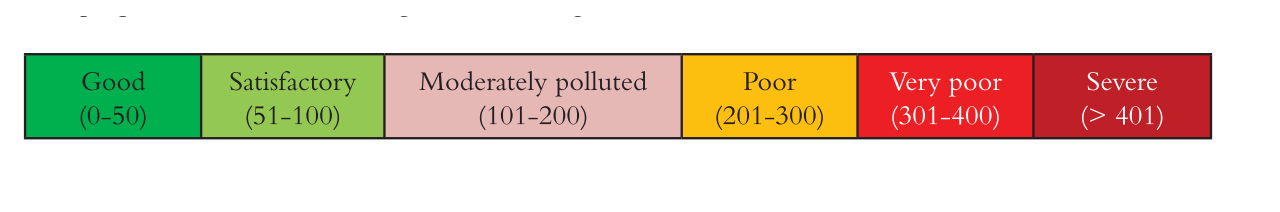
\includegraphics[scale=0.58]{./images/figure13.png}
    \end{center}
   
    \caption{Air Quality Index (AQI) \cite{AirQualityIndex}}
    
    \label{aqi}
\end{figure}

Health Canada and Environment Canada developed AQHI based five major pollutants 
$PM_{2.5}, O_3, NO_2, SO_2,$ and $CO$. Later the last two pollutants were dropped from the calculation as they were identified to  contribute very less in predicting health effects in Canada. AQHI computed using the following formula.


\begin{equation}
AQHI = \lceil (\frac{1000}{10.4}) \times [e^A-1]+[e^B-1]+[e^C-1] \rceil
\end{equation}

where $ A = 0.000537 \times$ concentration of  $O_3$, $B = 0.000871 \times$ concentration  of $NO_2$ and  $C = 0.000487 \times$ concentration of $PM_{2.5}$.
The value of AQHI varies from 1 to 10+ as shown in figure \ref{aqhi}


\begin{figure}[h]
    \begin{center}
    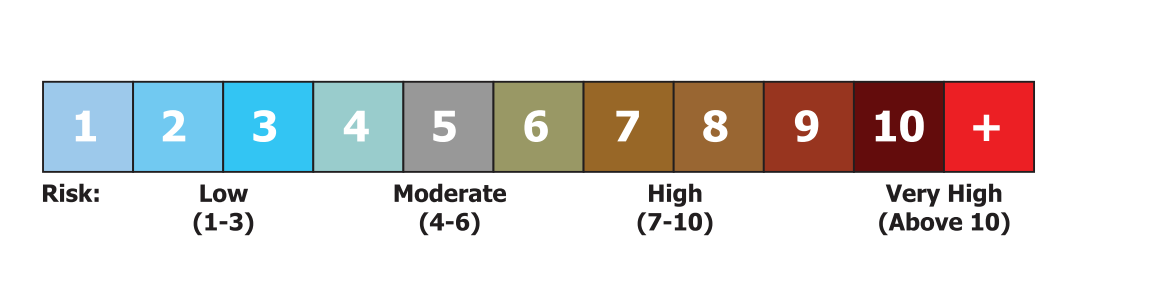
\includegraphics[scale=0.58]{./images/figure12.png}
    \end{center}
   
    \caption{Air Quality Health Index (AQHI) \cite{healthcanada}}
    
    \label{aqhi}
\end{figure}

Now the question is which is a better measure, AQI or AQHI? Since AQI is based on a single pollutant, it is hard to see its direct relationship with human health compared to AQHI \cite{Chen2013}. On the other hand AQHI is based on the relationship between the major air pollutant mix and mortality risk in 12 
Canadian cities, it is not clear it can be directly generalized to rural
areas or other cities across the world \cite{Chen2013}.



\section{Impact of Air Pollution}

Air pollution has significantly increased after the industrialization and urbanization have taken place. The burning of fossil fuels, exhaust from factories and industries, and mining operations are the major contributors to air pollution. The exposure to air pollutants causes premature deaths, cardiovascular disease, stroke, and other respiratory diseases. The state of global air 2017 has discussed the effects of long-term exposure to harmful air pollutants such as particulate matter which contributes to over 4 million premature deaths and is estimated to
double by 2050 if the issue remains unattended \cite{HealthEffectsInstitute2017}. Among the risk factors with the serious health issues, air pollution ranks the highest annually accounting for majority of deaths. The major impacts of air pollution are premature deaths, cardiovascular disease, stroke and other respiratory diseases.
Particles with a diameter of less than 10 microns ($PM10$), and less than 2.5 microns ($PM2.5$) causes the greatest threat to health, as they are capable of penetrating to lungs which leads to cardiovascular and chronic obstructive pulmonary diseases (COPD). \cite{who} \cite{Tian2016}. Exposure to carbon monoxide ($CO$) which is a colorless and odorless gas is absorbed into bloodstream from lungs and reduces the ability to transfer oxygen which inturn affects the functionality of organs such as brain and heart \cite{Sierra-vargas2012} \cite{Golbabaei2012}. Respiratory issues such as decrease in responsiveness of airways, inflammation in airways, lung infectivity occurs due to exposure of high concentration of ozone ($O3$) \cite{Lippmann1989}. Another pollutant is nitrogen dioxide ($NO2$) which causes such as wheezing, coughing, bronchitis and flu. The exposure of mixed air pollutants leads to diverse health effects like birth defects, development delays in children, skin irritation or even cancer \cite{MarilenaKampa2007}.

\section{Background}

The quality of the air has declined since the industrialization has taken place in the mid 19th century. Ever since then it has affected not just the environment but also the human health. There was a development of heavy industries across Europe to North America which used coal as their major source of energy that contributed to black smoke pollution \cite{Heidorn1978} \cite{Timothy}. Coal was not just used in industries but also in houses for heating in winter which made the pollution even worse \cite{Al2016}. These emissions resulted in serious health impacts on residents in urban areas that increased the mortality rate during this period. One such important event in the history of pollution is the great smog of London which killed as many as 12,000 people to death mostly infants. This was caused due to the combination of cold weather with smoke and lasted for several days \cite{londonfog}. There were a string of similar events reported in New York, England, Britain around the same time. All these incidents led to the development of Environmental Protection Agency (EPA) who enforced the need for installing the monitoring stations. The government along with these environmental agencies established acts like clean air act, motor vehicle air pollution act, air pollution control acts for a better quality of air\cite{airpollutionact}. 


\subsection{Existing Environmental Monitoring station}

The government and the environment agencies are taking an effort for installing monitoring stations for improving the air quality. The EPA monitors the criteria pollutants along with any special pollutant dominant in that particular area. At present there are two main methods for pollutant measurement: 1) passive sampling, and 2)active sampling \cite{Balakrishnan2015} \cite{activepassive}. These sampling techniques are considered as one of the most significant development for air quality measurement. These approaches are used widely for monitoring purpose. In passive sampling the pollutants are collected by physical process such as diffusion through a static air layer or membrane. pollutants contaminated in the air is diffused to adsorb on the sampling media.

\subsection{Low cost Sensor}







\section{Motivation}

One of the important components in solving this issue is to increase the awareness among public about the current situation and its impact so that they can act on it. The conventional method of monitoring the air quality with the help of a few heavyweight expensive stationary monitoring systems typically installed by the state may not be effective enough for this task. To achieve the goal effectively and without further delay, pollution monitoring must become part of daily activity for everyone. For that the devices to monitor pollution must be small, portable, inexpensive, and part of a global system. With the technological advancement of low cost computing, communication, and sensing devices, and the revolution and the importance of open source software \cite{Anthes2016}, we believe it is possible to build pervasive air pollution monitoring system with commodity hardware and open source software. Now the question is how to design such pollution monitoring devices faster and make them accessible to as many as possible. 
\\
Achieving the above stated goal requires a suitable system framework that can help to accelerate the process of the design and implementation of a air pollution monitoring system using the of-the-shelf commodity hardware and open source software. There are some recent attempts in this direction, but none is comprehensive and simple enough to follow and build a air pollution monitoring system with a little or moderate effort. This thesis is an attempt to fill that gap by first proposing a simple and comprehensive framework and then demonstrating its feasibility and use by creating our own pollution monitoring system that is operational in our lab. We have also added a step of calibration by implementing a web-based tool to find out the quality of data obtained from the system. Our contribution is a step towards inspiring and motivating not only the public to use the device, but also many amateur electronic hobbyists to buy the hardware locally and download the associated software to build their own pollution monitoring device.


\section{Research Problem}
The aim is to design and develop an air pollution monitoring system using off the shelf
hardware and open source software and analyze the quality of data obtained through calibration with the following objectives in mind.
\begin{enumerate}
    \item To develop a calibration tool which could give how accurate the sensor data is when compared with referance data.
    
    \item To educate the common people on adverse effect of air pollution by showing how polluted
    the vicinity is.
    
    \item To influence the behaviour of people by representing the concentration of pollutant as well
    as AQHI (Air Quality Health Index) which provides the seriousness that pollutants cause
    to health.
    
    \item To give an idea of how to integrate all the hardware components to a processor and also
    make an independent software, which can be accessed anywhere in the world.
    
    \item To encourage and help citizen science to solve the issue of air pollution and give more
    understanding to the impact it cause to human health and environment.

\end{enumerate}


\section{Thesis Contribution}

\section{Structure of the Thesis}